\section{OSI(Open Systems Interconnection)}

O OSI  ou Interconexão de Sistemas Abertos é um modelo usado para entender como os protocolos de rede funcionam. Para facilitar a interconexão de sistemas de computadores, a ISO (International Standards Organization) desenvolveu um modelo de referência chamado OSI (Open Systems Interconnection) para que os fabricantes pudessem criar protocolos a partir deste modelo. \cite{TORRESOSI}

Protocolo é uma “linguagem” usada para transmitir dados pela rede. Para que dois computadores passam se comunicar, eles devem usar o mesmo protocolo (ou seja, a mesma linguagem).

O modelo OSI é dividido em sete camadas. Cada camada é responsável por algum tipo de processamento e cada camada apenas se comunica com a camada imediatamente inferior ou superior. \cite{VENTURAOSI}

\begin{figure}[h]
  \centering
  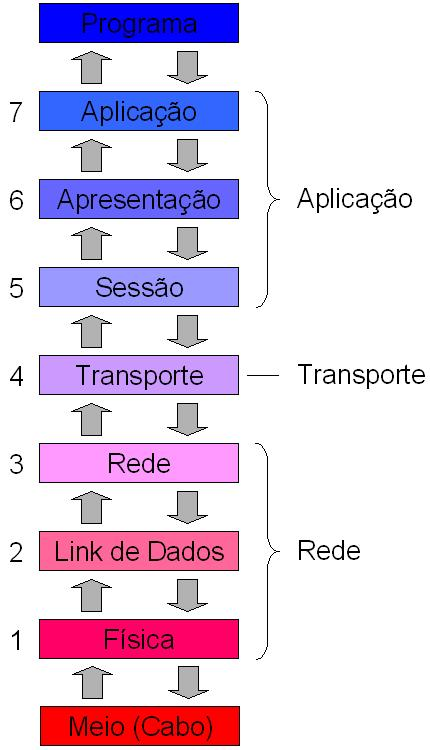
\includegraphics[scale=0.35]{img/camadas}
  \caption{\it As sete camadas OSI \cite{TORRESOSI}}
  \label{fig:CamadaOSI}
\end{figure}

A Figura \ref{fig:CamadaOSI} demostra a estrutura das camadas OSI. As sete camadas podem ser agrupadas em três grupos: Aplicação, Transporte e Rede:

\begin{itemize}
 \item \textbf{{Rede}} \\
	As camadas deste grupo são camadas de baixo nível que lidam com a transmissão e recepção dos dados da rede.
 \item \textbf{{Transporte}} \\
	Esta camada é responsável por pegar os dados recebidos da rede e transformá-los em um formato compreensível pelo programa. Quando seu computador está transmitindo dados, esta camada pega os dados e os divide em vários pacotes para serem transmitidos pela rede. Quando seu computador está recebendo dados, esta camada pega os pacotes recebidos e os coloca em ordem.
 \item \textbf{{Aplicação}} \\
	Essas são as camadas mais altas que colocam os dados no formato usado pelo programa.
\end{itemize}

Quando o computador está transmitindo dados, o fluxo da informação é do programa para a rede (isto é, o caminho de dados é de cima para baixo), portanto os programas se comunicam com a camada 7, que por sua vez se comunica com a camada 6 e assim por diante. Quando o computador está recebendo dados, o fluxo da informação é da rede para o programa (isto é, o caminho de dados é de baixo para cima), portanto a rede se comunica com a camada 1, que por sua vez se comunica com a camada 2 e assim por diante.

A seguir, serão descritas as características do protocolo IRC em cada uma das camadas:

\subsection{Camada Física}

Esta camada pega os quadros enviados pela camada de Link de Dados e os transforma em sinais compatíveis com o meio onde os dados deverão ser transmitidos. Se o meio for elétrico, essa camada converte os 0s e 1s dos quadros em sinais elétricos a serem transmitidos pelo cabo; se o meio for óptico (uma fibra óptica), essa camada converte os 0s e 1s dos quadros em sinais luminosos; se uma rede sem fio for usada, então os 0s e 1s são convertidos em sinais eletromagnéticos; e assim por diante.

%Acrescentar aqui a classificação do IRC nesta camada
% aqui é pelo meio em que é realizada a transmissão dos dados. Se são via internet, é dada pela via, seja ela por cabos ou wireless.

\subsection{Camada de Enlace ou Ligação de Dados}

Essa camada, também chamada camada de Enlace, pega os pacotes de dados recebidos da camada de rede e os transforma em quadros que serão trafegados pela rede, adicionando informações como o endereço da placa de rede de origem, o endereço da placa de rede de destino, dados de controle, os dados em si e uma soma de verificação, também conhecida como CRC(Cyclic Redundancy Check) ou verificação de redundância cíclica, que é um código detector de erros. O quadro criado por esta camada é enviado para a camada Física, que converte esse quadro em sinais elétricos (ou sinais eletromagnéticos, se a rede for sem fio) para serem enviados através do cabo de rede. Quando o receptor recebe um quadro, a camada de Link de Dados confere se o dado chegou íntegro, refazendo a soma de verificação (CRC). Se os dados estiverem corretos, ele envia uma confirmação de recebimento chamada acknowledge(admitido ou reconhecido). Caso essa confirmação não seja recebida, a camada Link de Dados do transmissor reenvia o quadro, já que ele não chegou até o receptor ou então chegou com os dados corrompidos.

%Acrescentar aqui a classificação do IRC nesta camada
% é o meio por onde são realizadas as comunicações entre o client/server sever/client. Seja por mensagens ou transferências de arquivos.

\subsection{Camada de Rede}

Esta camada é responsável pelo endereçamento dos pacotes, convertendo endereços lógicos em endereços físicos, de forma que os pacotes consigam chegar corretamente ao destino. Essa camada também determina a rota que os pacotes irão seguir para atingir o destino, levando em consideração fatores como condições de tráfego da rede e prioridades.

%Acrescentar aqui a classificação do IRC nesta camada
% faz com que a mensagem ou arquivo direcionado à alguém conectado ao servidor, chegue ao seu destino.

\subsection{Camada de Transporte}

Nas redes de computadores os dados são divididos em vários pacotes. No computador receptor, esses pacotes são organizados para formar o arquivo originalmente transmitido. A camada de Transporte é responsável por pegar os dados enviados pela camada de Sessão e dividí-los em pacotes que serão transmitidos pela rede. Isso inclui controle de fluxo (colocar os pacotes recebidos em ordem, caso eles tenham chegado fora de ordem) e correção de erros, tipicamente enviando para o transmissor uma informação de reconhecimento (acknowledge), informando que o pacote foi recebido com sucesso.

%Acrescentar aqui a classificação do IRC nesta camada
% é nesta camada onde os pacotes recebidos são organizados afim de obter o arquivo original que foi enviado. Pode ser tanto pela comunicação em mensagens quanto para a troca de arquivos.

\subsection{Camada de Sessão}

Esta camada permite que dois programas em computadores diferentes estabeleçam uma sessão de comunicação. Nesta sessão, esses dois programas definem como será feita a transmissão dos dados e coloca marcações nos dados que estão sendo transmitidos. Se porventura a rede falhar, os dois computadores reiniciam a transmissão dos dados a partir da última marcação recebida em vez de retransmitir todos os dados novamente.

%Acrescentar aqui a classificação do IRC nesta camada
% hum... eu pensei que talvez pudesse ser a questão da situação da pessoa (algo tipo se está on-line, ocupada, etc)... algo que tenha como vínculo uma comunicação direta. Acho que essa vc precisará pensar um pouquinho hehe.

\subsection{Camada de Apresentação}

Também chamada camada de Tradução, esta camada converte o formato do dado recebido pela camada de Aplicação em um formato comum a ser usado pela pilha de protocolos. Se o programa está usando um código de página diferente do ASCII por exemplo, esta camada será a responsável por traduzir o dado recebido para o padrão ASCII. Esta camada também pode ser usada para comprimir e/ou criptografar os dados. A compressão dos dados aumenta o desempenho da rede, já que menos dados serão enviados para a camada inferior (camada 5). Se for utilizado algum esquema de criptografia, os dados circularão criptografados entre as camadas 5 e 1 e serão descriptografadas apenas na camada 6 no computador de destino.

%Acrescentar aqui a classificação do IRC nesta camada
% aqui podemos falar sobre segurança das informações, onde podem ser utilizadas criptografias para evitar que arquivos e conversas sejam interceptadas.

\subsection{Camada de Aplicação}

A camada de aplicação faz a interface entre o programa que está enviando ou recebendo dados e a pilha de protocolos. É onde há a comunicação entre usuário e máquina, para que os seres humanos sejam capazes de obter informações por meio de uma interface mais amigável.

%Acrescentar aqui a classificação do IRC nesta camada
% No caso do IRC, são os clients, programas cuja interface torna possível a troca de informações entre outros usuários conectados.